%%%%%%%%%%%%%%%%%%%%%%%%%%%%%%%%%%%%%%%%%%%%%%%%%%%%%%%%%%%%%%%%%%%%
%% I, the copyright holder of this work, release this work into the
%% public domain. This applies worldwide. In some countries this may
%% not be legally possible; if so: I grant anyone the right to use
%% this work for any purpose, without any conditions, unless such
%% conditions are required by law.
%%%%%%%%%%%%%%%%%%%%%%%%%%%%%%%%%%%%%%%%%%%%%%%%%%%%%%%%%%%%%%%%%%%%

\documentclass{beamer}
\usetheme[faculty=fi]{fibeamer}
\usepackage[utf8]{inputenc}
\usepackage[
  main=slovak %% By using `czech` or `slovak` as the main locale
                %% instead of `english`, you can typeset the
                %% presentation in either Czech or Slovak,
                %% respectively.
  %% The additional keys allow foreign texts to be
]{babel}        %% typeset as follows:
%%
%%   \begin{otherlanguage}{czech}   ... \end{otherlanguage}
%%   \begin{otherlanguage}{slovak}  ... \end{otherlanguage}
%%
%% These macros specify information about the presentation
\title{Analýza inštalačných APK súborov pre OS Android} %% that will be typeset on the
\subtitle{Bakalárska práca} %% title page.
\author{Martin Styk}
%% These additional packages are used within the document:
\usepackage{ragged2e}  % `\justifying` text
\usepackage{booktabs}  % Tables
\usepackage{tabularx}
\usepackage{tikz}      % Diagrams
\usetikzlibrary{calc, shapes, backgrounds}
\usepackage{amsmath, amssymb}
\usepackage{url}       % `\url`s
\usepackage{listings}
\usepackage{fancybox}
\usepackage{tikz}
\usepackage{pgf-pie}
\usepackage{longtable}
\usepackage{tabularx}
\usepackage{bchart} 
 % Code listings
\frenchspacing
\begin{document}
  \frame{\maketitle}
%  \AtBeginSection[]{% Print an outline at the beginning of sections
%    \begin{frame}<beamer>
%      \frametitle{Outline for Section \uv{\insertsectionhead}}
%      \tableofcontents[currentsection]
%    \end{frame}}

\section{Ciele práce}
  \begin{frame}[label=lists]{Ciele práce}
    \begin{itemize}
    \item Vytvoriť rozsiahlu databázu inštalačných súborov pre OS Android (APK súborov)
	\item Popísať štruktúru a formát inštalačných súborov
	\item Vytvoriť nástroj na analýzu a získavanie metadát o inštalačných súboroch
	\item Určiť štatistické informácie o aplikáciách vo vytvorenej databáze
	\item Implementovať mechanizmus detekcie potenciálne modifikovaných APK súborov
    \end{itemize}  
  \end{frame}

%\subsection{OS Android}
%  \begin{frame}[label=lists]{OS Android}
%    \begin{itemize}
%    \item 84,7\% podiel na trhu s mobilnými operačnými systémami \cite{marketshare}
%\item Obľúbenosť vďaka veľkému počtu aplikácií
%\item Riziko jednoduchej možnosti modifikácie inštalačných súborov
%    \end{itemize}  
%  \end{frame}  
  
\section{Databáza inštalačných súborov}
  \begin{frame}[label=lists]{Databáza inštalačných súborov}
    \framesubtitle{Uvažované zdroje APK súborov}
    \begin{itemize}
    \item Oficiálne zdroje
    	\begin{itemize} 
    	\item Obchod s aplikáciami Google Play Store 
    	\end{itemize}
    \item Neoficiálne zdroje
    	\begin{itemize}
    	\item Neoficiálne obchody s aplikáciami
    		\begin{itemize}
    		\item SlideMe
    		\item Amazon Appstore 
			\end{itemize}    	 
    	\end{itemize}
    	\begin{itemize}
    	\item Stránky na zdieľanie obsahu
    		\begin{itemize}
    		\item ZippyShare
    		\item UlozTo 
			\end{itemize}    	 
    	\end{itemize}
    	\begin{itemize}
    	\item Torrenty
    	\end{itemize}
    \end{itemize}  
  \end{frame}  
  
%   \begin{frame}[label=lists]{Získavanie aplikácií z Google Play}
%    \begin{itemize}
%  		\item Možné len do zaregistrovaného Android zariadenia
%  		\item Aplikácia Google Play Crawler \cite{crawler}
%  		\item Projekt Playdrone
%  			\begin{itemize}
%  			\item Databáza 1\,100\,000 APK súborov z Google Play
%			\item November 2014
%  			\item Apk súbory dostupne vo verejnom archíve
%  			\end{itemize}
%    \end{itemize}  
%  \end{frame}  

  \begin{frame}[label=lists]{Databáza inštalačných súborov}
    \framesubtitle{Automatizácia hromadného preberania APK súborov}
    \begin{itemize}
  		\item Implementovaný nástroj ApkDownloader\cite{apkdownloader}
  		\item Založený na princípe analýzy HTML kódu
  		\begin{itemize}
  		\item Vyhľadanie priamych odkazov na APK súbory
  		\item Prevzatie APK súborov
  		\end{itemize}
		\item Implementovaný pre nasledujúce lokality
  		\begin{itemize}
  			\item archív projektu Playdrone
	  		\item www.appsapk.com
  			\item www.apkmaniafull.com
  			\item ww.androidapksfree.com
  		\end{itemize}
  		\item Jednoducho rozšíritelný, open source
    \end{itemize}  
  \end{frame}  
  
  \begin{frame}[label=lists]{Databáza inštalačných súborov}
    \framesubtitle{Výsledná databáza APK súborov}
	\begin{itemize}
	\item Celkovo získaných 20\,060 APK súborov, z toho viac ako 90\,\% pomocou ApkDownloader
		\item Celková veľkosť prebraných APK súborov 192\,GB
\end{itemize}	    
    
    \begin{table}[htb]
\centering
  \begin{tabular}{l r r}
    
    \textbf{Zdroj} & \textbf{Počet aplikácií} & \textbf{\%} \\\hline
    Playdrone & 8\,200 & 40,9\\
    www.appsapk.com & 6\,470 & 32,3\\
    www.apkmaniafull.com & 2\,870 & 14,3\\
    www.androidapksfree.com & 1\,030 & 5,1\\
    www.zippyshare.com & 750 & 3,7\\
    torrenty & 550 & 2,7\\
    www.uloz.to & 190 & 0,9\\
    \hline
    Spolu & 20\,060 & \\
  \end{tabular}
 % \caption{Zdroje prevzatých APK súborov}
  \label{tab:stahovanie}
\end{table}
  
\end{frame}  
  
  %%%%%%%%%%%%%%%%%%%%%%Struktura APK /ANALYZA 

\section{Analýza inštalačných APK súborov}
  \begin{frame}[label=lists]{Analýza inštalačných APK súborov}
   \framesubtitle{Štruktúra a formát APK súborov}
    \begin{columns}
      \column{.55\textwidth}
       \begin{itemize}
		\item Slúžia na distribúciu aplikácií na platforme Android
		\item Android application package file	
		\item Štruktúra vychádza z formátu JAR
		\item Archívne súbory vo formáte ZIP
		\item Typicka štruktúra s povinnými súbormi v pevne stanovenom formáte
		\item Niektore súbory v nečitateľnej skompilovanej podobe
	\end{itemize}	  
      \column{.45\textwidth}
        	 \begin{figure}[htb]
    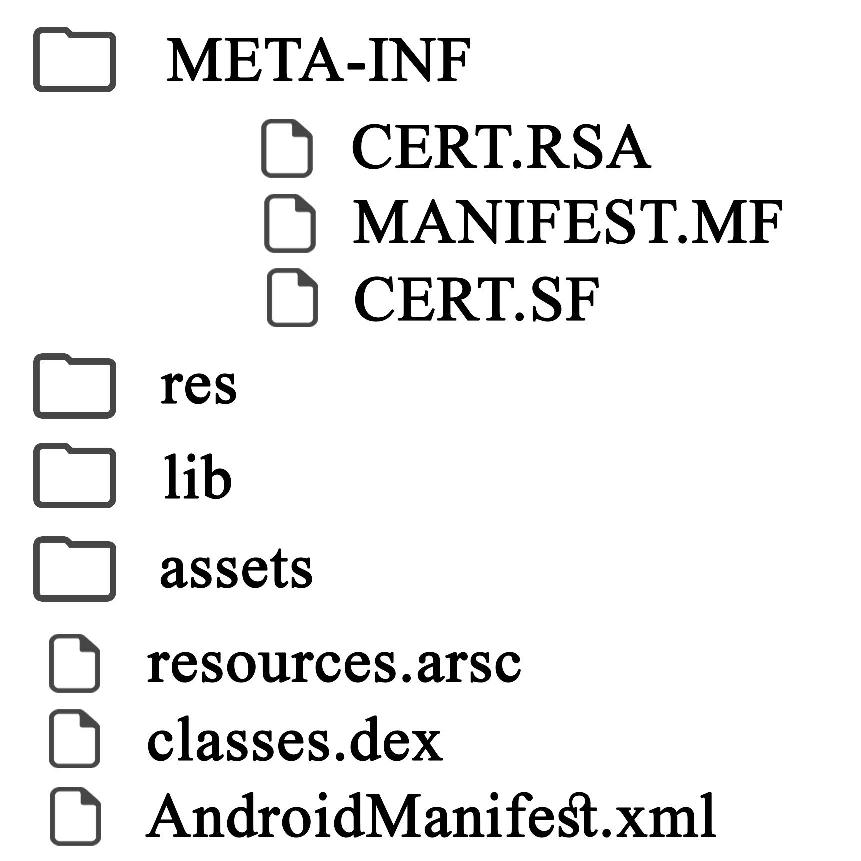
\includegraphics[width=45mm]{images/apkStructure.pdf}
  \label{fig:strukturaApk}
\end{figure}
    \end{columns}
    
   \end{frame} 
    
  \begin{frame}[label=lists]{Analýza APK súborov}
  \framesubtitle{Implementácia analýzy}
	\begin{itemize}
		\item Cieľom získanie detailných metadát o rôznych aspektoch APK súborov
		\item Automatizované pomocou vyvinutej aplikácie ApkAnalyzer\cite{apkanalyzer}
		\item Využitie nástroja ApkTool na dekompiláciu \cite{apktool}
		\item Použitá knižnica AXML na konverziu binárnych XML súborov do čitateľnej formy \cite{axml}
		\item Celkovo získaných 63 atribútov každého APK súboru
	\end{itemize}	    
   \end{frame} 
   
   
   \begin{frame}[label=lists]{Analýza APK súborov}
  		\framesubtitle{Príklady zbieraných informácií}
	 \begin{itemize}
			\item Základné informácie
			\begin{itemize}
				\item veľkosť APK súboru, veľkosti dôležitých súborov
			\end{itemize}
			\item Dáta zo súboru AndroidManifest.xml
			\begin{itemize}
				\item komponenty aplikácie
				\item prístupové oprávnenia
				\item verzia Android SDK
			\end{itemize}
			\item Informácie o certifikáte
			\begin{itemize}
				\item algoritmus podpisu
			\end{itemize}
			\item Informácie o zdrojových súboroch
			\begin{itemize}
				\item formáty obrázkov
				\item lokalizácia
			\end{itemize}
			\item Hashe jednotlivých súborov
		\end{itemize}	    
   \end{frame} 

\subsection{Štatistiky nad databázou APK súborov}
  \begin{frame}[label=lists]{Štatistiky nad databázou APK súborov}
  \framesubtitle{Najčastejšie prístupové oprávnenia}
	 \begin{table}[!htbp]
\centering
  \begin{tabular}{l r}
    \textbf{Názov} & \textbf{\%} \\\hline
    android.permission.internet & 92,9 \\
    android.permission.access\_network\_state & 87,9 \\
    android.permission.write\_external\_storage & 75,2 \\
    android.permission.wake\_lock & 49,5 \\
    android.permission.read\_phone\_state & 49,4 \\
    android.permission.access\_wifi\_state & 44,7 \\
    android.permission.vibrate & 43,6 \\
    android.permission.get\_accounts & 31,3 \\
    android.permission.receive\_boot\_completed & 30,5 \\\hline
  \end{tabular}
  %\caption{Najpoužívanejšie prístupové oprávnenia}
  \label{tab:permissions}
\end{table}
  \end{frame} 
  
  
  \begin{frame}[label=lists]{Štatistiky nad databázou APK súborov}
  \framesubtitle{Algoritmus podpisu APK balíčka}
\begin{figure}[H]
\centering
\begin{bchart}[min=0,max=80,step=10,unit=\%]
\bcbar[label=MD2withRSA]{0.01}
\bcskip{6pt}
\bcbar[label=SHA512withRSA]{0.06}
\bcskip{6pt}
\bcbar[label=SHA1withDSA]{3.60}
\bcskip{6pt}
\bcbar[label=MD5withRSA]{5.88}
\bcskip{6pt}
\bcbar[label=SHA256withRSA]{15.56}
\bcskip{6pt}
\bcbar[label=SHA1withRSA]{74.87}
\bcskip{3pt}
\end{bchart}

\label{fig:signAlg}
\end{figure}
  \end{frame} 

     \begin{frame}[label=lists]{Štatistiky nad databázou APK súborov}
  \framesubtitle{Lokalizácie aplikácií}
\begin{table}[htb]
\centering
  \begin{tabular}{l l r}
    \textbf{Kód} & \textbf{Jazyk} &  \textbf{\%} \\\hline
    es & španielsky & 61,7 \\
    de & nemecký & 59,6 \\
    fr & francúzsky & 59,4 \\
    ru & ruský & 58,1 \\
    ja & japonský & 57,6 \\
    it & taliansky & 57,4 \\
	ko & korejský & 56,9 \\
	zh-rcn & čínsky (zjednodušený) & 55,6\\
    \hline
  \end{tabular}
  \label{tab:language}
\end{table}
\begin{itemize}
\item Anglický jazyk považovaný za základ, nevyskytuje sa v tabuľke.
\item V českom jazyku je lokalizovaných 49\,\% aplikácií, v slovenčine 46\,\%
\end{itemize}
\end{frame}

\section{Detekcia prebalených APK súborov}
  \begin{frame}[label=lists]{Detekcia prebalených APK súborov}
 	 \framesubtitle{Možnosti a hrozby modifikácie APK súborov}
	\begin{itemize}
	 	\item Apk súbory je možné rozbaliť, modifikovať a zabaliť do pôvodnej podoby
	 	\item Android obsahuje ochranný mechanizmus
	 	 \begin{itemize}
	 	 	\item súbor MANIFEST.MF obsahuje hash každého súboru - ochrana 	integrity
		 \end{itemize}	 
		 \item Jednoduché vyhnutie ochrannému mechanizmu 
	 	 \begin{itemize}
	 	 	\item po každej zmene nutné balíček podpísať
		 \end{itemize}	 
		 \item Spôsob šírenia malvéru	  
	\end{itemize}
  \end{frame} 
  
  \begin{frame}[label=lists]{Detekcia prebalených APK súborov}
 	 \framesubtitle{Detekcia prebalených APK súborov}
	\begin{itemize}
	 	\item Implementovaná metóda detekcie nadmieru podobných APK súborov pomocou podobnosti súborov a metadát o aplikáciách
	 	\item Malvérové aplikácie zachovávajú look \& feel pôvodných
	 	\item Funkcionalita obsiahnutá v aplikácií ApkAnalyzer
	 	\item Vyuzitie metadát získaných analýzou APK súborov
	 	\item Párové porovnanie APK súborov
	\end{itemize}
  \end{frame} 

    \begin{frame}[label=lists]{Detekcia prebalených APK súborov}
 	 \framesubtitle{Navrhnutá metóda detekcie prebalených APK súborov}
	\begin{figure}[htb]
  \begin{center}
    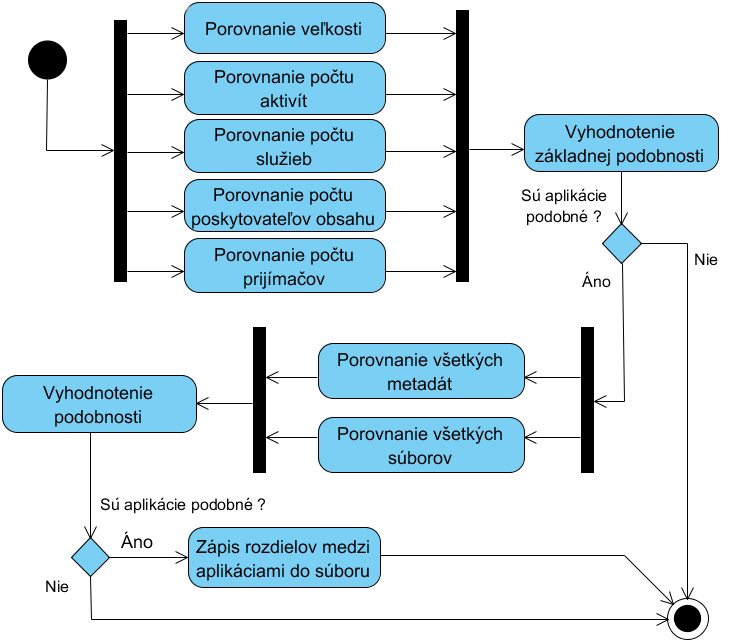
\includegraphics[height=6.5cm]{images/diagram.jpg}
  \end{center}
\end{figure}
  \end{frame} 

  \begin{frame}[label=lists]{Detekcia prebalených APK súborov}
   \framesubtitle{Výstup}
	\begin{itemize}
	\item Výstup párového porovnania obsahuje detailné rozdiely medzi jednotlivými aplikáciami
	\item Na základe zhody certifikátu a verzie aplikácie sú vyhodnotené potenciálne škodlivé aplikácie
	\item Identifikovaných 161 nadmieru podobných APK súborov s rovnakou verziou podpísaných rôznymi certifikátmi
	\end{itemize}
	\end{frame}


  \begin{frame}[label=bibliography]{Bibliografia}
    \framesubtitle{Analýza inštalačných APK súborov pre OS Android}
    \begin{thebibliography}{9}
      \bibitem{marketshare}
         www.gartner.com/newsroom/id/3169417.
      \bibitem{crawler}
          https://github.com/Akdeniz/google-play-crawler
      \bibitem{apkdownloader}
          github.com/MartinStyk/ApkDownloader
      \bibitem{apkanalyzer}
          github.com/MartinStyk/ApkAnalyzer
      \bibitem{apktool}
          ibotpeaches.github.io/Apktool/
      \bibitem{axml}
          axml
    
    \end{thebibliography}
  \end{frame}
\end{document}
